\documentclass[a4,11pt]{article}

\parindent=10pt
\parskip=6pt
%\usepackage[width=15.5cm, left=2.5cm, top=2cm, height= 24.5cm]{geometry}

\usepackage[paper=a4paper, left=2cm, right=2cm, bottom=2.5cm,top=2.5cm]{geometry}

% Paquetes de nacionalización. No olvidar para poder poner tildes!
\usepackage[spanish]{babel}
\usepackage[utf8]{inputenc}

% Paquetes para graficos
\usepackage{subfig}
% \usepackage{graphicx} %% La caratula lo incluye

% Paquetes para matematica
\usepackage{amsmath}
\usepackage{amsfonts}
\usepackage{amssymb}
% esto es para el codigo
\usepackage{listings}
% Paquetes para pseudo
\usepackage{algorithm}
\usepackage{algorithmic}

% Caratula (Recordar logo_uba.jpg y logo_dc.jpg)
\usepackage{caratula}

% Paquetes para tablas
\usepackage[table]{xcolor}

% Se pueden sacar?
\usepackage{url}
\usepackage{float}
\usepackage{afterpage}
\usepackage{tabularx}

% Color de links
\usepackage{hyperref}
\hypersetup{
    colorlinks,
    citecolor=black,
    filecolor=black,
    linkcolor=black,
    urlcolor=black
}

\lstset{
    language=C++,
    basicstyle=\ttfamily,
    breaklines=true,
    breakatwhitespace=true,
    inputencoding=utf8,
    extendedchars=true
    }
\lstset{literate={::}{}{0\discretionary{::}{}{::}}% line-break at ::
   {->}{}{0\discretionary{->}{}{->}}% line-break at ->
}

\begin{document}


\materia{Metodos numericos}
\submateria{Primer Cuatrimestre de 2016}
\titulo{Re entrega Trabajo Pr\'actico 2}
\subtitulo{“CSI:DC”}
\integrante{ Ricardo Colombo}{156/08}{ricardogcolombo@gmail.com}
% keywords
\providecommand{\keywords}[1]{\textbf{\textit{Palabras Claves---}} #1}

\maketitle
\pagebreak
\begin{abstract}
 A lo largo de este trabajo abarcaremos distintas tecnicas y estrategias utilizadas en machine learninng intentando dar con la mas adecuada para obtener la mejor clasificacion de un conjunto de digitos manuscritos basandonos en la informacion mas relevante de cada una de ellas con el fin de poder realizar un reconocimiento.

\end{abstract}

\keywords{Machine Learning, Reconocimientos de digitos, Analisis de componentes principales. Regresion de minimos cuadrados}


\tableofcontents

\pagebreak
El objetivo de este trabajo práctico es desarollarar un clasificador que permita reconocer dígitos manuscritos.
Par llevarlo a cabo analizaremos técnicas de reconocimiento óptico de caracteres (OCR). Es un proceso dirigido a la digitalización de caracteres manuscritos, los cuales identifican automáticamente a partir de una imagen símbolos o caracteres que pertenecen a un determinado alfabeto, para luego almacenarlos en forma de datos.

Exploraremos la técnica de reconocimiento K-NN, K vecinos más próximos, además experimentaremos con distintas variantes de clasificación:

\begin{itemize}
\item PCA
\item PLSDA
\end{itemize}


Luego analizaremos la performance de cada una de estas técnicas mediante un set de experimentos, para evaluar las fortalezas y deficiencias de cada una de ellas. \\


\subsection{Introducción Teórica}


\subsubsection{Reconocimiento óptico de caracteres}


La tecnología de reconocimiento de caracteres, OCR (Optical Character  Recognition)  engloba  a  un  conjunto  de  téc
nicas basadas en  estadísticas, en las formas de los caracteres, transformadas y en comparaciones, que complementánd
ose entre sí, se  emplean para  distinguir de forma automática entre  los diferentes caracteres alfanuméricos existentes.
Enrealidad no se reconocen  exactamente los  caracteres de un determinado alfabeto, sino que es posible distinguir entre cualquier conjunto de formas o símbolos. Sin embargo, se debe tener en cuenta que la precisión que se obtiene en la práctica al inten
tar distinguir entre un conjunto de símbolos no es total. Por lo tanto, es fácil  deducir  que  cuanto  más  numeroso  es  el conjunto de símbolos entre los que se debe decidir, mayor es la probabilidad de que se produzca un fallo de clasificación. 
En todo sistema de reconocimiento óptico de caracteres se distinguen al menos estas 4 etapas: 

\begin{itemize}
\item Preproceso 
\item Segmentación 
\item Extracción de características 
\item Reconocimiento 
\end{itemize}


\subsubsubsection{Preproceso}

En esta fase de preprocesamiento (o adecuación de la imagen) el objetivo que se persigue es eliminar de la imagen de cualquier 
tipo de ruido o imperfección que no pertenezca al carácter, así como normalizar el tamaño del mismo. La normalización de la imagen también puede implicar un binarizado de la misma. Para la eliminación del ruido que puede aparecer en una imagen digital se utilizan diversos algoritmos:
\begin{itemize}
\item Etiquetado:  para  la  división  de  la  imagen  en  regiones  de componentes conectadas. 
\item Erosión / expansión: para la eliminación de peque\~nos grupos de píxeles. 
\item Umbralizado de histograma:  para  eliminar/seleccionar los objetos más brillantes o más oscuros de la imagen.  
\end{itemize}


\subsubsubsection{Segmentación}

Una vez preprocesada la imagen se deberá segmentar en las diferentes componentes conexas (parte de la imagen donde todos los píxeles son adyacentes entre sí) que la componen. La segmentación de la imagen constituye una de las mayores dificultades del reconocimiento, y se hace  necesaria para poder reconocer cada uno de los caracteres de la imagen binaria.
La fragmentación o segmentación es la operación que permite la descomposición  de  un  texto  en  diferentes  entidades lógicas. Estas entidades deben ser lo suficientemente invariables, para ser independientes del escritor, y lo suficientemente significativas para su reconocimiento.  


\subsubsubsection{Extracción de características}

Una  vez  realizada  la  segmentación,  se  tiene  una  imagen normalizada en la que se encuentra la información susceptible de ser “reconocida”. La información así representada, una matriz bidimensional de valores binarios.

La extracción de las características es una de las fases  más difíciles, dado que es muy difícil elegir un conjunto de características óptimo. 
Para que una característica se pueda considerar buena debe tener: 
\begin{itemize}
\item Discriminación: Deben  ser características que diferencien suficientemente una clase de otra
\item Deben tener igual valor para mismas clases 
\item Independencia: Las características deben estar incorreladas unas de otras. 
\item Pequeño espacio para características: El número de características debe ser pequeño para la rapidez y facilidad de clasificación. 
\end{itemize}

En este trabajo desarrollaremos y evaluaremos dos técnicas.


{\ttfamily PCA (Principal Component Analysis)} 

El objetivo de esta técnica es definir una transformación lineal desde el espacio de representación original a un nuevo espacio en el que las distintas clases de las muestras quedan mejor separadas.
Esta transformación permite reducir la dimensión del nuevo espacio sin perjudicar sensiblemente la capacidad discriminativa de la nueva representación. 

{\ttfamily PSL-DA (Partial Least Squares Discriminant Analysis)} 

Es un método estadístico que tiene relación con la regresión de componentes principales, se encuentra una regresión lineal mediante la proyección de las variables de predicción y las variables observables a un nuevo espacio. Debido a que tanto los datos de X e Y se proyectan a nuevos espacios, los familia de los modelos PLS se conoce como factor de modelos bilineales. Los cuadrados mínimos parciales Análisis discriminante (PLS-DA) es una variante que se utiliza cuando la Y es binaria.


\subsubsubsection{Reconocimiento}

Una  vez  se  tienen  las  características  más  importantes de la imagen a analizar hay que determinar el  carácter correspondiente en este trabajo exploraremos la técnica de KNN.


\subsubsection{ K-NN (K vecinos más próximos)}

Es un método no paramétrico y supervisado, que dado un conjunto de objetos prototipo de los que ya se conoce su clase (es decir, dado un conjunto de caracteres de muestra) y dado un  nuevo objeto cuya clase no conocemos (imagen de un carácter a reconocer) se busca entre el conjunto de prototipos los “k” más parecidos a nuevo objeto. A este se le asigna la clase más numerosa entre los “k” objetos prototipo seleccionados.  


\subsubsubsection{Entrenamiento y Test}


Conociendo el funcionamiento básico del método de clasificación de los “k vecinos más próximos” es obvio que para poder empezar a trabajar con este método es necesario reunir un conjunto de datos etiquetados, es decir, un conjunto de muestras prototipo con las clases a las que pertenecen. Esta recolección implica disponer de una base de datos de imágenes de los tipos de caracteres que posteriormente se esperen reconocer. A este conjunto de datos se le denomina conjunto de entrenamiento. Sin embargo, la fase de entrenamiento no solo consiste en la recopilación de estos datos, sino que, típicamente, los datos originales que se dedican al 
entrenamiento deben ser preprocesados adecuadamente para obtener representaciones compactas y coherentes. Esto quiere decir que  las  imágenes deben ser segmentadas, normalizadas y transformadas para obtener los vectores de baja dimensionalidad que finalmente se almacenan como conjunto de entrenamiento.
Con este conjunto de entrenamiento ya construido, el clasificador “knn” ya puede ser utilizado para reconocer la clase de una nueva muestra. Esta es la fase de test y lógicamente, también aquí es necesario aplicar todo el preproceso descrito anteriormente a cada una de las nuevas muestras. Por lo tanto, aquí se ve la necesidad de disponer de métodos rápidos de realizar estas tareas de preproceso, puesto que la velocidad de reconocimiento dependerá, en parte, de ellos. En la práctica se tiene que este preproceso es posible realizarlo muy rápidamente, aunque justo a continuación aparece la parte del proceso de reconocimiento que normalmente más carga computacional conlleva, la clasificación. 





\pagebreak
\subsection{Entrada y salida de los algoritmos}

Dados los requirimientos de la catedra el programa toma como parametros 3 argumentos, el primero es el archivo de entrada, luego el archivo de salida y
por ultimo el modo.  La catedra solicitaba 3 modos el modo 0,1 y2 para los 3 metodos solicitados, luego agregamos 3 modos mas utilizados durante la etapa de expermentacion.

\begin{enumerate}
    \item Eliminacion Gaussiana(EG)
    \item Factorizacion de Cholesky(CL)
    \item WP
    \item Cholesky con modificacion de partidos jugados
    \item Cholesky haciendo ganar al ultimo con el siguiente reiteradas veces hasta quedar primero
    \item Cholesky haciendo ganar al ultimo con el primero del ranking hasta quedar primero
\end{enumerate}

El modo 3 modo corre cholesky y luego busca 2 equipos que hayan jugado previamente para cambiar su resultado y luego volver a ejecutar cholesky,
para este modo se puede ingresar un parametro mas donde se indica la cantidad de partidos que se deben jugar de nuevo.

Para el modo 4 corre cholesky y luego ejecuta un ciclo donde el objetivo es lograr que el que haya salido ultimo luego de obtener el ranking de cholesky llegue al primer puesto ganandole
al que tiene por arriba inmediato en el ranking. En cada paso agrega un partido mas y vuelve a calcular cholesky para la nueva matriz, asi obtenemos un nuevo ranking y continuamos iterando hasta quedar en la primera posicion, siempre utilizando al que salio ultimo en la primera utilizacion del metodo de cholesky.
Una vez finalizado por stdout devuelve la cantidad de partidos jugados, ademas de que en el archivo  rankingSTEPS_4.out dentro de la carpeta test se encuentran los rankings en cada iteracion y como es la evolucion.
El modo 5 es similar al anterior con la sutil diferencia que el participante que salio ultimo la primera vez que corrio cholesky llegue al primer puesto jugandole al que se encuentra en el primer puesto en cada iteracion.


Tanto el formato de entrada y de salida del programa son los solicitados por la catedra.
Para todos los metodos el archivo de entrada es el mismo, que contiene el siguiente formato:
\begin{pmatrix}
 (n) & (k) \\
 (x1) & (e1) & (r1) & (t1) & (s1)\\
 (x2) & (e2) & (r2) & (t2) & (s1)\\
...\\
 (xk) & (ek) & (rk) & (tk) & (s1)\\
\end{pmatrix}

la primer linea tiene 2 valores $n$ representa la cantidad de equipos y $k$ representa la cantidad de partidos, seguido k lineas que representa cada partido, donde
$x1$ representa una fecha que en nuestro caso no utilizamos, luego $ei$ y $ti$ representan los numeros de los equipos, y por ultimo $ri$ y $s1$ representan las anotaciones de cada equipo respectivamente.
en nuestra experimentacion con fines de no complejizar aum mas el problema no utilizamos en campo que representa la fecha si no que asumimos que dado el orden que venian los resultados era el orden de los partidos.

Luego una vez se ejecutan los metodos 0-4 devuelven un archivo de n lineas donde en la linea se obtiene el ranking del equipo i. 

Para los metodos 4 y 5 se devuelve el ranking para cada iteracion antes de jugar el partido, estas se repiten hasta que el que comenzo ultimo termine primero utilizando dos metodos descriptos anteriormente, en la ultima linea se obtiene la cantidad total de partidos,
estos dos metodos ademas devuelven por stdout la cantidad de partidos jugados hasta que termino en la primer posicion el que comenzo ultimo.



\subsection{Sistema a resolver}

\[ C_{i,j} =
    \begin{cases}
        n_{i,j}       & \quad \text{si }  \text{i $\neq$ j}\\
        2+n_i & \quad \text{si } \text{ i $\eq$ j }\\
    \end{cases}

    \]
Esta matriz es simetrica y definida positiva y ademas es estrictamente diagonal domimante.
Por lo tanto es posible hallar la factorizacion de Cholesky , que no es mas que un caso
de factorizacion LU , esto nos permite asegurar que a la hora de hacer eliminacion 
gaussiana no vamos a hallar 0 en la diagonal , con lo cual no hace faltar considerar
pivoteo parcial en la eliminacion Gaussiana.  

%Las Caracteristicas de esta matriz son -La Matriz es Simetrica y definida positiva
%-Es estrictamente Diagonal Domimante  
%-Por lo tanto se le puede hacer la factorizacion de Cholesky que no es mas que
%un caso particular de Factorizacion LU
%-Si se le puede hallar la factorizacion LU , eso significa que la eliminaion gausiana
%no va a hallar 0 en la diagonal , con lo cual no hace falta considerar pivoteo en el algoritmo
%-El metodo para crear la matriz esta basado en la regla de metodos sucesivos de LaPlace
    


\subsection{Método Matriz de Colley}

Para la implementación de esta técnica nos basamos en el paper \textbf{The Colley Matrix Explained}. La cual consiste en plantear un sistema de ecuaciones

La principal fortaleza de este método es que es útil para obtener rankings en torneos donde los participantes no juegan la misma cantidad de partidos. Además de que al armar el sistema en base a los resultados pasados, da relevancia al calendario de juegos de cada participante. Como se intentará demostrar en la sección de experimentos, utilizando esta tecnica importa contra quien se gana y contra quien se pierde. Además tiene el atractivo de que da una idea sobre la posibilidad de victoria en el siguiente partido, considerando los partidos anteriores. \\

La principal desventaja y que hace que no sea aplicable a muchos de los deportes es que los empates no pueden ser modelados. \\

Una vez obtenida la \textbf{Matriz de Colley} vamos a  presentar dos técnicas de resolucion del sistema de ecuaciones solicitado. \\

\subsubsection{Eliminación Gaussiana}
La implementación del algorimo de \textbf{Eliminación Gaussiana} que elegimos es la que se encuentra en el libro \textbf{Burden[1]}.Con el agregado de backgward substitution para obtener el vector de la ecuacion Cr=b.

\begin{algorithm}
    \begin{algorithmic}[1]\parskip=1mm
        \caption{vector Gauss(matriz A, vector b)}
        \STATE{Para k=$1...n-1$}\\
        \STATE{\quad Para i=$1...n-1$}\\
        \STATE{\quad\quad Tomo el elemento $a_{k,k}$ como pivot}\\
        \STATE{\quad\quad Para $j = i+1,...n$}\\
        \STATE{\quad \quad \quad $a_{i,j}  = a_{i,j} - a_{i,j} * (a_{i,k} / a_{k,k})$}\\
        \STATE{\quad \quad \quad $b_{i}  = b_{i} - a_{i,j} * (a_{i,k} / a_{k,k})$}\\
        \STATE{$x_{n} = a_{n,n+1}/a_{n,n}$}\\
        \STATE{para $i=n-1..1$}\\
        \STATE{\quad para $j=i+1..n$}\\
        \STATE{\quad\quad $ sum +=a_{i,j}*x_{j}$}\\
        \STATE{devolver x}
    \end{algorithmic}
\end{algorithm}

Para este algoritmo como se puede observar es de complejidad O($n^3$) en el peor caso, ya que en ciclo interno de las posiciones 4 a 6 se ejecuta n veces y el ciclo de las lineas 2 a 6 se ejecuta n veces por lo tanto ya tendriamos n^2 iteraciones en el peor caso y finalizando con el ciclo de las lineas 1 a 6 que se ejecuta otras n veces.
Luego en las lineas 7 a 10 se realiza el backgward substitution  que tiene en el peor caso se ejecuta $n^2$ veces.

\subsubsection{Cholesky}

La implementación del algorimo de \textbf{Eliminación Gaussiana} que elegimos es la que se encuentra en el libro \textbf{Burden}.
Agregandole los pasos que mensiona en el libro (pagina 420) para resolver el sistema Cr=b.

\begin{algorithm}
    \begin{algorithmic}[1]\parskip=1mm
        \caption{vector Cholesky(matriz A, vector b)}
        \STATE{$l_{1,1} = \sqrt{a_{1,1}$}}\\
        \STATE{Para $j = 2,...n$}\\
        \STATE{\quad $ l_{j,1} = a_{j,1} / l_{1,1}$}\\
        \STATE{Para $i = 2,...n-1$}\\
        \STATE{\quad $l_{i,i}  = (a_{i,i} - \sum_{k=1}^{i-1}{l^2_{i,k}}^{1/2})$}\\
        \STATE{\quad Para $j = i+1,...n1$}\\
        \STATE{\quad\quad $l_{j,i}  = (a_{j,i} - \sum_{k=1}^{i-1}{l_{j,k} l_{i,k}} / l_{i,i})$}\\
        \STATE{$l_{n,n}  = (a_{n,n} - $\sum_{k=1}^{n-1}{l^2_{n,k}}}\\
        \STATE{y_1$=$b_1\l_{1,1}\\
        \STATE{Para i$=$2..n}\\
        \STATE{\quad Para j$=$1..i-1}\\
        \STATE{\quad\quad sum$=$l_{i,j}*y_j}\\
        \STATE{\quad\quad y_i$=$(b_i-sum)\l_{i,i}}\\
        \STATE{x_n$=$y_n\l_{n,n}\\
        \STATE{Para i$=$n-1..1}\\
        \STATE{\quad Para j$=$i+1..n}\\
        \STATE{\quad\quad sum$=l_{i,j}*x_j$}\\
        \STATE{\quad\quad x_i$=$(y_i-sum)\l_{i,i}}\\
        \STATE{devolver x}
    \end{algorithmic}
\end{algorithm}\\


\subsection{Porcentaje de Victorias}

La primer técnica es \textbf{Porcentaje de Victorias} que a lo largo del análisis denominaremos \textbf{WP} que consiste en tomar el promedio de partidos ganados / partidos jugados. 
Esta técnica basicamente analiza la performance de un equipo participante en los partidos jugados en base a partidos ganados. \\

En este caso el score de un equipo no es afectado por la cantidad de partidos y resultados obtenidos de los demás participantes, pero esto si afecta su posición final en el ranking. \\

Esta técnica a priori no aporta mucha informacion respectoa la posibilidad de victoria en el siguiente encuentro y tampoco considera el ranking del rival enfrentado.
Ya que todos los partidos valen lo mismo. \\

La implementación consiste en calcular: $\sum_{i=1}^n{} \frac{G_i}{T}$ \\

Sonde \textbf{n} es la cantidad de partidos jugados, \textbf{G} corresponde a partidos ganados y \textbf{T} al total de partidos jugados. \\


\pagebreak
\section{Experimentacion y resultados}

Para analizar los algortimos implementados vamos a utilizar varios archivos de test generados por nosotros, los cuales estan mas detallados en el apendice, con el fin de realizar una serie de test que nos permitirán en primer caso encontrar parametros buenos con lo que ejecutar los distintos metodos y posteriormente evaluar el desempeño de la implementación mediante las métricas propuestas por la cátedra.

Dividimos la experimentación en dos secciones, una para cada archivo de prueba. Y evaluaremos los parametros individualmente para cada una de ellas

\subsection {Algoritmo de K-NN}

Lo primero que vamos a hacer es encontrar un valor de $K$ que nos permita maximizar la cantidad de aciertos, sin tener en consideración las métricas.

Ejecutamos el algoritmos de $K-NN$ variando los valores de k entre {1..30} dejando fija la cantidad de particiones para $K=$6 y $K=$15. Luego para cada una de las iteraciones tomamos el promedio, esto se utilizo tanto para la cantidad de aciertos como para la cantidad de vecinos.

Cada uno de los conjuntos conto con 4200 imagenes a testear. En los siguientes graficos presentamos algunos de los sets obtenidos:

Expresamos los aciertos para cada K en con el siguiente gráfico:
\begin{center}
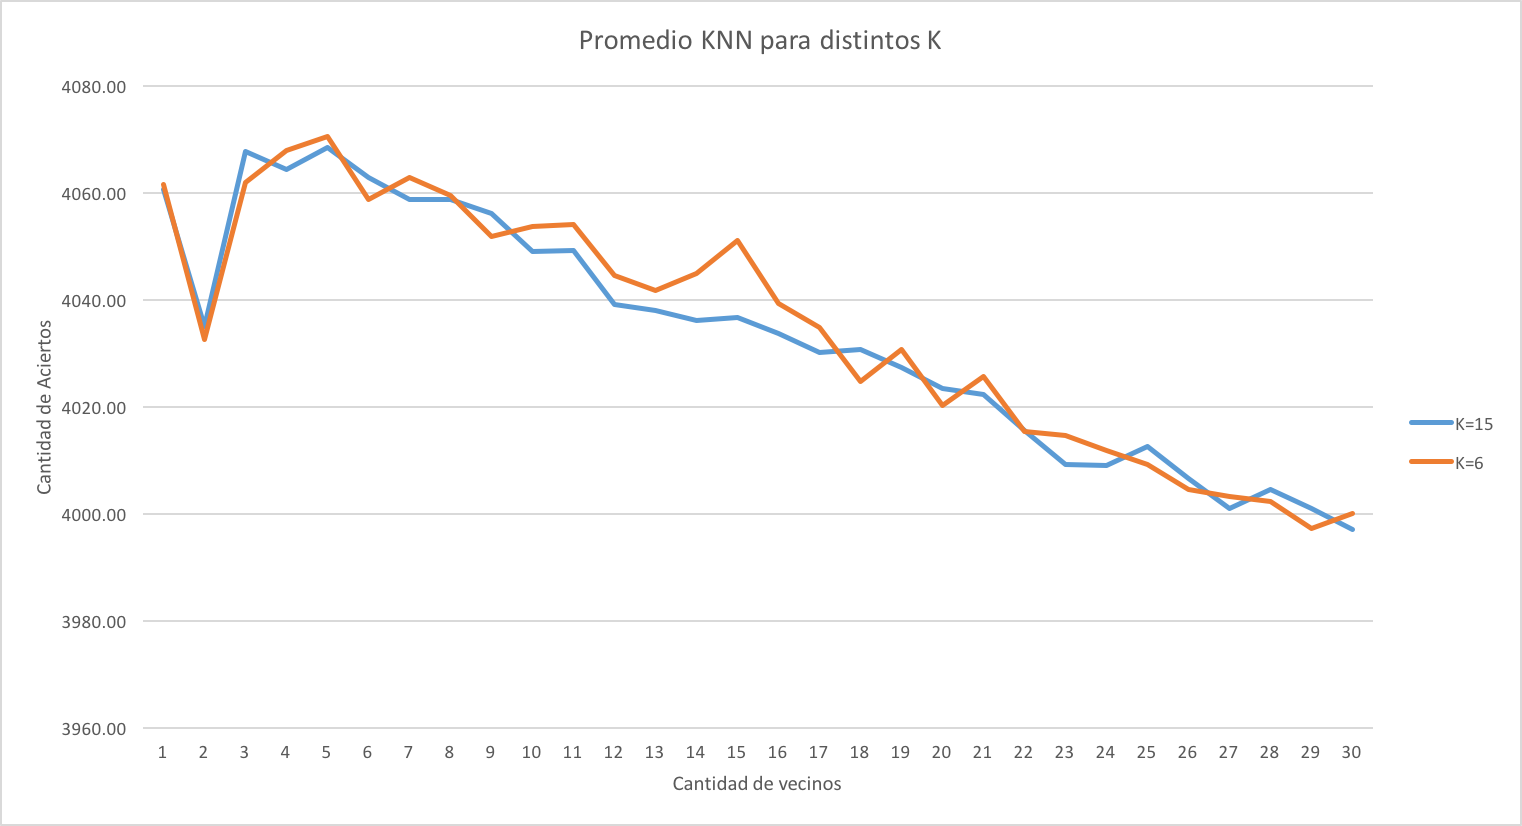
\includegraphics[scale=0.6]{imagenes/AciertosKNN.png}
\end{center}

Como se puede observar para ambos $K$ tienen el mismo patron a lo largo que se incrementa la cantidad de vecinos $k$, pero ambas parecen alcanzar un maximo en $k=5$ como cantidad de vecinos. Además notemos que a medida que se incrementa el valor de $k$ la cantidad de aciertos va disminuyendo levemente, cumpliendo lo mencionado en el desarrollo. Cuanto mas corta sea la distancia de los vecinos, mas chances hay de tener un acierto sin importar el valor de $K$.

Si nos detenemos y obsvervamos con mas claridad cuando para la combinacion de $K$=6 y $k$=5 es donde se maximizan en comparativa para knn, lo que intentaremos hacer en los proximos metodos es utilizar esta convinacion de $K$=6 y ir variando la cantidad de vecinos mas cercanos para ver si existe algun tipo de relacion con el fin de asegurar que esa convinacion es la mejor.

Por otro lado hicimos un analisis temporal para saber como afectaba la cantidad de particiones que tomamos para el cross validation y variamos la cantidad de vecinos tomados para ver como se comportaba, los cuales arrojaron los siguientes resultados. 

\begin{center}
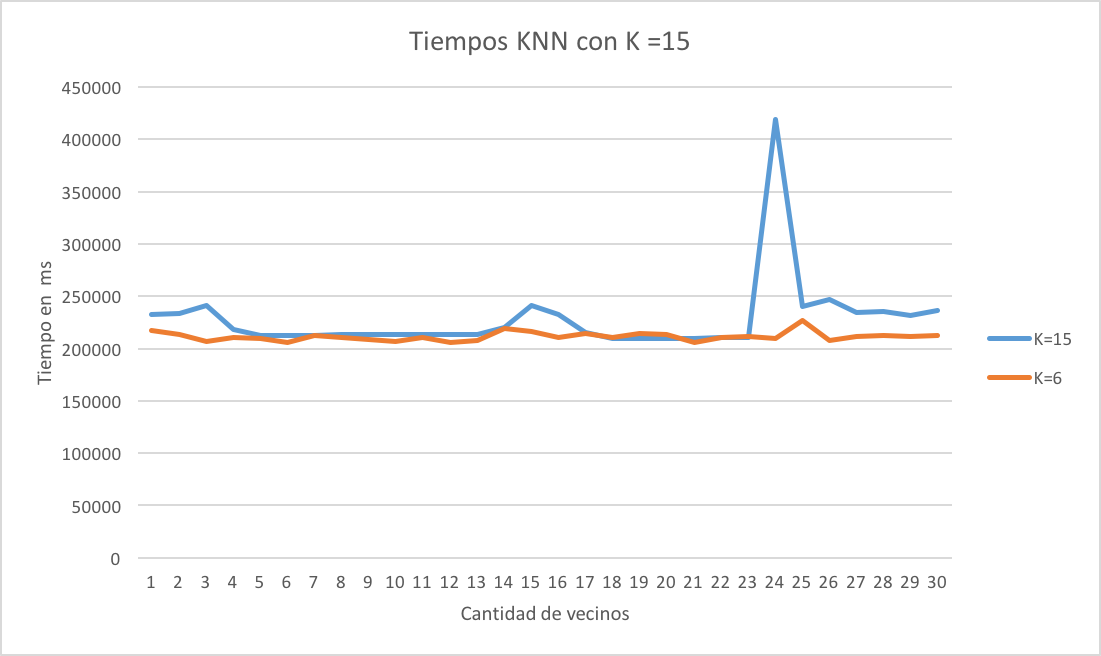
\includegraphics[scale=0.6]{imagenes/TiemposKNN.png}
\end{center}

En cuanto a los tiempos para diferentes $K$ no varian mucho en la media, si bien se puede notar al principio que a mayor cantidad de ejecuciones mayor es el tiempo que demora, algo prevesible previamente. Lo que notamos es que hay un pico cuando tomamos entre 23 y 25 vecinos mas cercanos.Sin embargo,esto es un caso que deberiamos seguir ejecutando para esos parametros con el fin de ver si no es ruido que se pudo haber generado por otro proceso en el momento de la ejecucion para descartar esto.


\subsection {Algoritmo de K-NN con Optimización de PCA}
Para el algoritmo de PCA lo que realizamos fue una variacion de los valores de lambda (cantidad de componentes principales) en el algoritmo de pca. Para esos valores de $K$ medimos los tiempos de ejecución y los promediamos para poder ver de que manera varía la ejecución de los algoritmos en función de $\alpha$, luego tomamos un promedio de las ejecuciones y obtuvimos lo siguientes resultados:

\begin{center}
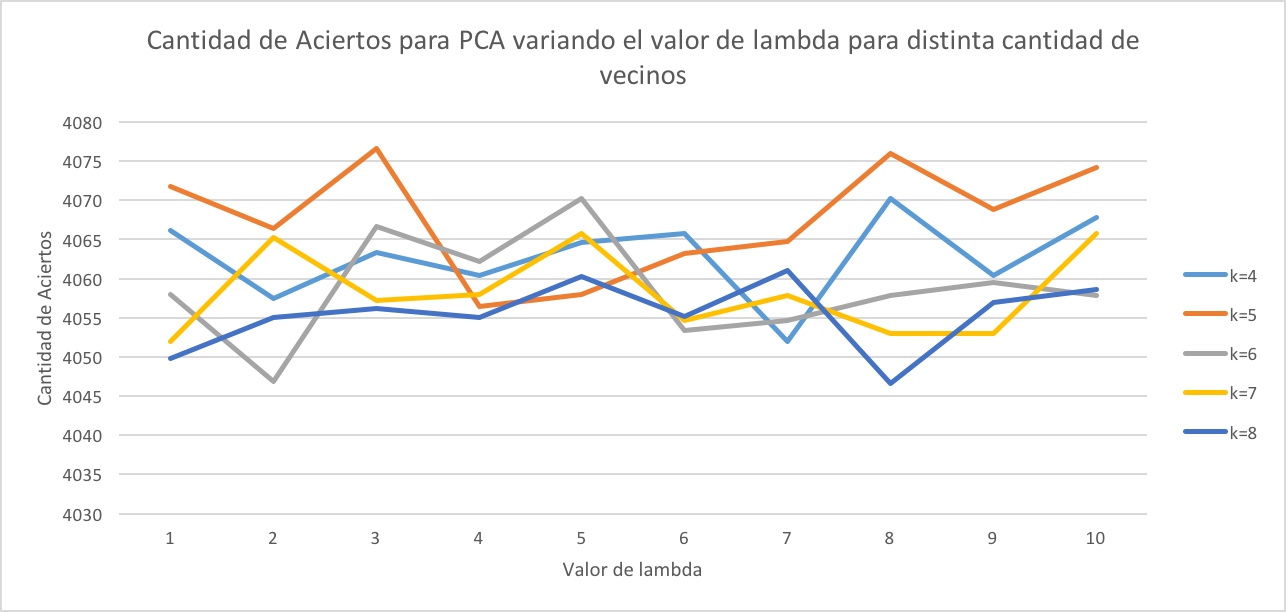
\includegraphics[scale=0.6]{imagenes/AciertosPCA.png}
\end{center}

Al ver estos resultados notamos a comparacion de los resultados obtenidos para KNN con $k$=5 se respetan para la optimizacion, ya que mirando las comvinaciones de lambda con cantidad de vecinos el que resulta como 'ganador' arrojando una cantidad de aciertos mayor a 4075 es cuando $k$=5 y $\lambda$=3. 

A medida crecia el lamda no parece llegar a igualarlo pero si esta muy cerca cuando se toman 8 componentes principales. 

\begin{center}
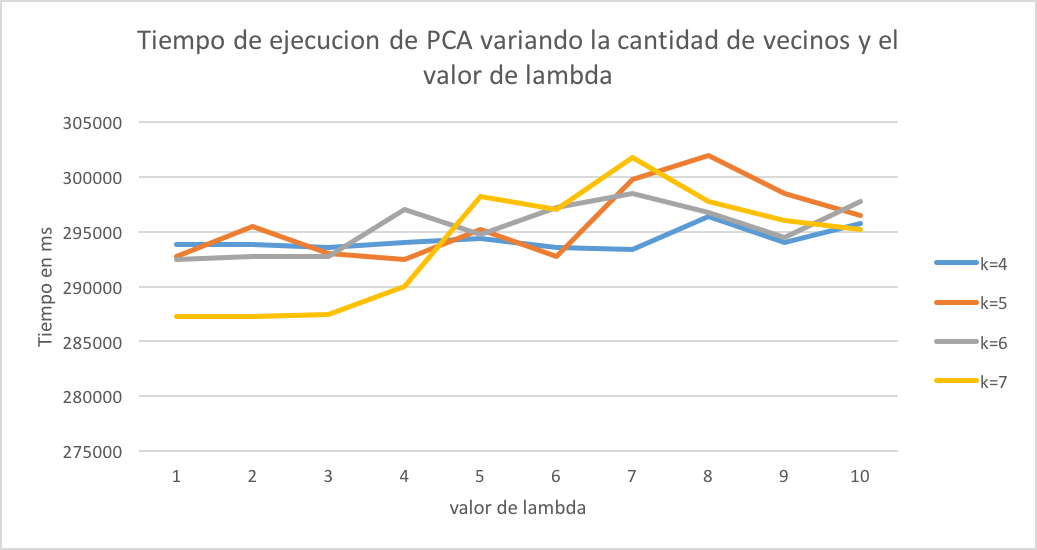
\includegraphics[scale=0.6]{imagenes/TiemposPCA.png}
\end{center}

En cuanto a los tiempos podemos cabe aclarar que estos tiempos no contemplan todo lo que se considera el ’entrenamiento’ del sistema, es decir, todo el preprocesamiento que resultara en encontrar
los valores principales. La justificacion de esto es que el procedimiento se realizar ́a una vez, para entrenar el sistema y luego, al momento de clasificar las
nuevas imagenes este tiempo podra ser despreciado.Este grafico se puede ver que aumentar el α produce un aumento lineal de los tiempos de ejecucion, 
de lo que se desprende que aumentar la cantidad valores principales no resulta gratuito en terminos de tiempo de ejecucion y tiene cierto costo asociado.

De igual manera la distribucion de tiempos al variar el lamda parece ir creciendo levemente y podriamos predecir que asi va a hacer mientras mas grande sea el valor de lambda.

\subsection {Algoritmo de K-NN con Optimización de PSL-DA}
Habiendo fijado k = 3 , corremos el test1.in variando el gamma utilizando los valores 1,2,10 y 50. Aqui el grafico
\begin{figure}[H]
\centering
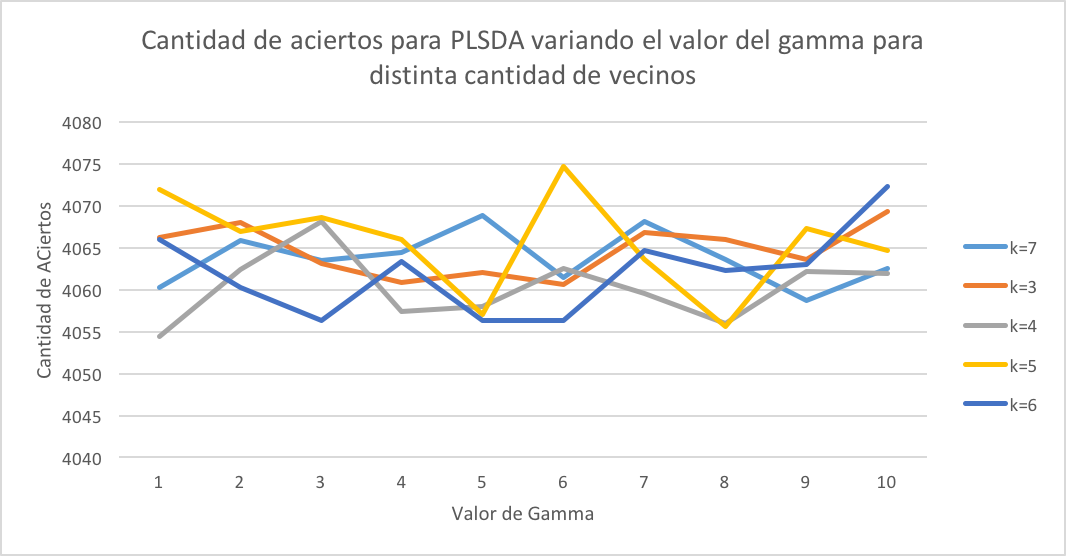
\includegraphics[width=1\textwidth]{imagenes/AciertosPLSDA.png}
\caption{Comparacion de aciertos variando el gamma}
\label{fig:Comparacion de tecnicas}
\end{figure}


\begin{center}
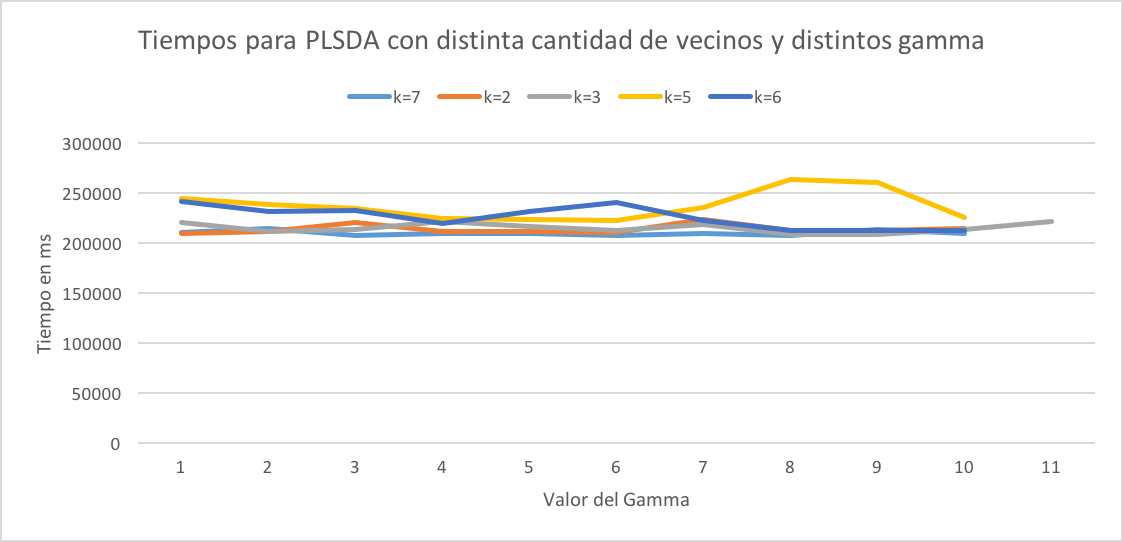
\includegraphics[scale=0.6]{imagenes/TiemposPLSDA.png}
\end{center}

Vemos que si aumenta el gamma , mejora la precision pero si gamma aumenta demasiado , en algun momento empeora tu hit rate , suponemos que eso se debe a que si bien tenemos bastante informacion , la cantidad de vecinos no permite aprovecharla . Eso hace suponer que para que tengamos un buen hit rate , debe haber algun tipo de relacion entre el k y el gamma . Eso se va a poner a prueba usando el test2.in

\subsection {Precision, recall y F1 Score para los mejores resultados obtenidos}

El ultimo de los puntos pedidos con el fin de analizar la calidad de los resultados obtenidos era la utilizacion de 2 metricas de las presentadas en el enunciado. Para nuestros experimentos decidimos usar Presicion y Recall.

Presicion se basa en la cantidad de aciertos relativos dentro de una clase particular. Osea, dada una clase $i$, definimos a los verdaderos positivos como $tp_i$ y los falsos positivos como $fp_i$, estos son aquellos que fueron definidos como una clase a la cual no pertencian.
Con lo cual la presicion de dicha clase se define como \\
\frac{$tp_i$}{$tp_i$+$fp_i$} 

Recall es una medida para saber que tan bueno es un clasificador para identificar a los que pertenecen a una clase, asumiendo que $fn_i$ son aquellos falsos negativos.
El Recall de una clase esta definido como \\
\frac{$tp_i$}{$tp_i$+$fn_i$} 

Luego para la mejor cantidad de vecinos obtenida (k=5); buscamos los valores de las metricas obtenidas para PCA.

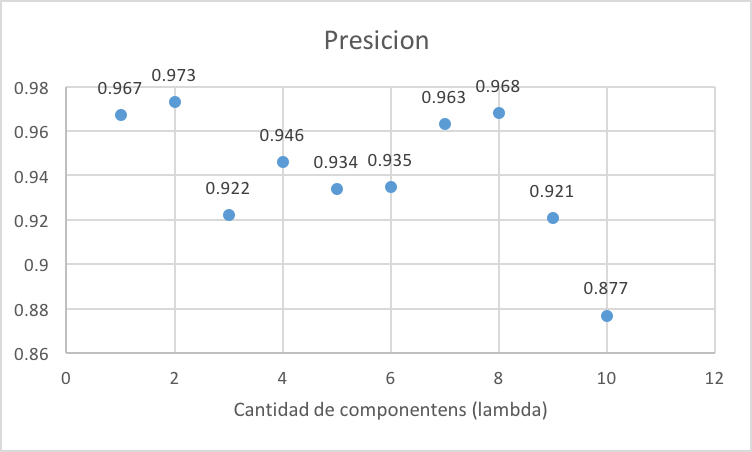
\includegraphics[scale=1]{imagenes/pcaPresicion.png}\\
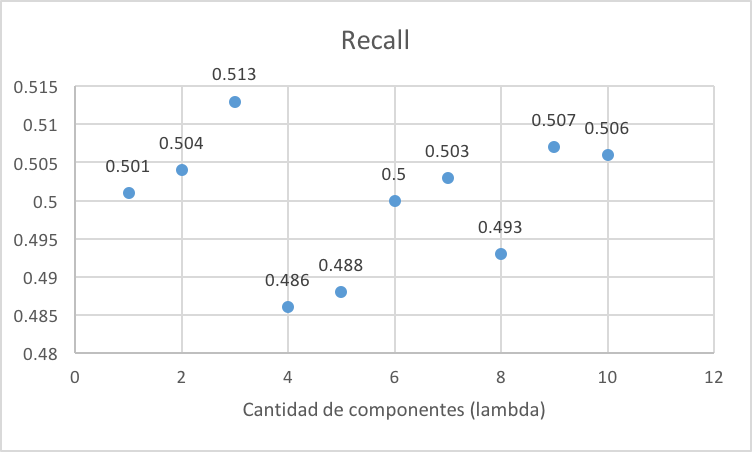
\includegraphics[scale=1]{imagenes/pcaRecall.png}

Como podemos ver los resultados para las metricas dieron muy parecidos en cuanto al lambda elegido para obtener el maximo dentro de la metrica. Sin embargo, esto esta basado en que la cantidad de vecinos que tomamos es 5 dado a que en los experimentos de KNN+PCA demostrados con anterioridad fue con la cantidad de vecinos el cual obtuvimos los mejores resultados.

Por otro lado repetimos el analisis para PLSDA con el fin e analizar las mismas metricas

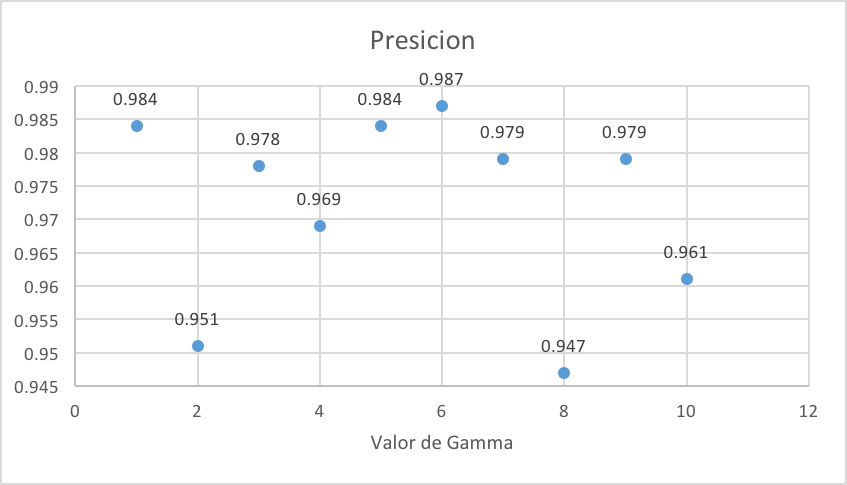
\includegraphics[scale=1]{imagenes/plsdaPresicion.png}\\
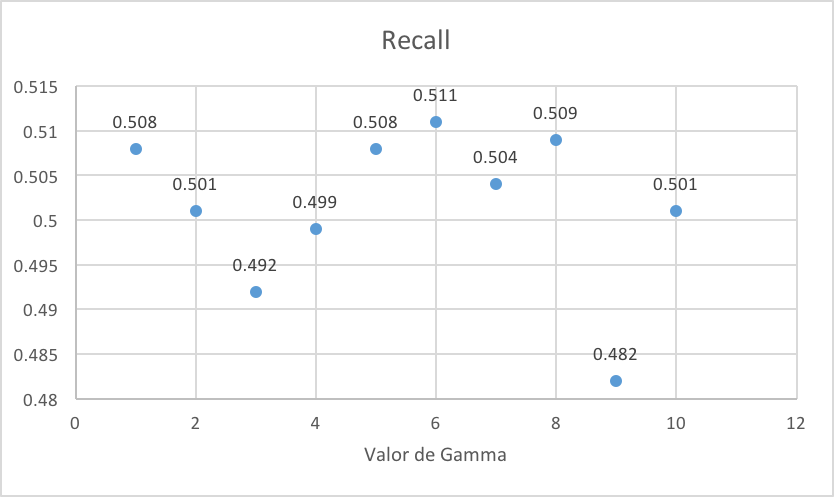
\includegraphics[scale=1]{imagenes/plsdaRecall.png}

En este caso podemos sacar la misma conclusion que en el caso anterior en cuanto a que las metricas para la combinacion de \gamma y $k$ con la cual se maximiza es la misma que para la cantidad de aciertos. 




% \pagebreak
% \section{Discusión}
% \subsection{Discusión}


\subsubsection{Ranking}

De los resultados obtenidos podemos ver que el ranking obtenido con \textbf{WP} no es muy realista, ya que la primer posición es ocupada por un participante que jugo y gano un solo partido. \\

El ranking obtenido por \textbf{CMM} refleja de forma mucho mas realista el desempeño de cada jugador en el torneo. \\

En un escenario donde tenemos participantes que jugaron una cantidad distinta de partidos pensamos que refleja mejor la realidad del torneo el metodo de \textbf{CMM}. \\


\subsubsection{¿Importa contra quien se pierde?}

Como podemos observar realmente importa contra quien se pierde, del experimento realizado observamos que perder contra el participante último afecta mas el puntaje del ranking que perdiendo contra el primero. \\

La hipótesis con la que calculamos el experimento resulto ser falsa. Analizando más ejecuciones llegamos a la conclusión de que lo resultados obtenidos son lógicos, ya que con esta técnica es mas esperable que un equipo de mitad de tabla tenga un resultado adverso contra los primeros, por lo cual la perdida de ranking es menor. \\


\subsubsection{Racha ganadora}

Por lo visto el jugador escalo rapidamente en la tabla de posiciones, y ademas mejoro el ranking de los participantes que lo vencieron a el.\\

Si bien mejoro su posición en la tabla, no alcanzo el top ten, y en las últimas victorias su ascenso fue mas lento. Esto nos hace concluir que solo haciendo jugar y ganar a un participante, la capacidad que tiene para crecer en el ranking esta limitada por la falta de juego de sus rivales.



\subsubsection{Escalando Posiciones}

\subsubsubsection{El torneo ya finalizo}

Poner resultados


\subsubsubsection{Agregando partidos}

Poner resultados



\subsubsubsection{Análisis Cuantitativo}

Como era de esperar en el caso de \textbf{WP} para instancias el tiempo de ejecución fue el mismo, y el tiempo demorado a medida que crecian los datos de la instancia fue lineal.

En cambio en el caso de \textbf{CMM} la implementación de \textbf{Cholesky} fue mas eficiente para las mismas instancias, y relativamente mejor a medida que se incrementaban los datos. Esto es esperado ya que nuestras implementaciones se basaron en las propuestas por el libro \textbf{Burden}, que afirma que \textbf{Cholesky} consume \frac{1}{3} n^3 flops y \textbf{Eliminación Gaussiana} \frac{2}{3} n^3 flops.


\subsubsubsection{La aritmética importa}

De los experimentos realizados notamos que es importante el tipo de datos utilizados. Principalmente cuando se utiliza \textbf{CMM}.
\\

Los errores de redondeo pueden derivar en un mal cálculo del ranking. Es decir, no considerar los suficientes decimales puede derivar en que un participante con un ranking decimalmente menor quede mejor rankeado que otro con mayor puntaje.\\

Por ejemplo: El participante A con ranking 0,5819 y el participante B con ranking 0,5816 si se consideran solo dos decimales ambos tienen 0,58 y esto podria afectar su orden en el ranking global. \\

Para evitar esta situacion nuestra implementación usa el tipo de datos float con con 5 decimales despues de la coma.\\


\subsubsubsection{Empates}

Encontramos que los empates pueden modelarse en el caso de \textbf{WP}, asignando un puntaje al partido empatado y continuando con el procedimiento normal.

En el caso de \textbf{CMM} nos resulto muy díficil tratar de modelarlo, como alternativa a este resultado proponemos modelarlo como si ambos equipos perdieran. Esto nos permite reutilizar el método y de alguna forma penar a ambos equipos por no haber ganado su partido.


















% \pagebreak
% \section{Conclusiones}

% \section{Conclusiones}


% \pagebreak
% \section{Apéndice}

% \subsection{Archivos de test usados}
Dentro de la carpeta /src/tests se encuentran los siguientes archivos usados en la experimentaci\'on
\begin{itemize}
 \item ATP2007.in este archivo es usado en la experimentaci\'on de escalar posici\'ones gandandole al siguiente o al primero del ranking
 \item ATP2007_100.in este archivo se utilizo en el analisis de salto de posici\'ones en cuanto a 100 partidos jugados para obtener una cota
 \item test1.in archivo provisto por la materia
 \item test2.ina archivo de prueba provisto por la materia
 \item carpeta random test tiene todos los archivos de test que se utilizaron para la medici\'on de tiempos
\end{itemize}



% \pagebreak
% \section{Bibliografía}
% \subsection{Bibliografía}

\begin{itemize}
 \item Numerical Analysis, Richard L. Burden \& J. Douglas Faires, Chapter 6: Direct Methods for Solving Linear Systems.
 \item Paper The Colley Matrix Explained http://www.colleyrankings.com/matrate.pdf.
\end{itemize}

% \pagebreak
% \section{Codigo}
% \subsection{Sobre los archivos e implementacion}

Para la implementacion de los archivo se utilizo C++, la siguiente es la lista de archivos y consecutivo a la misma hay una descripcion sobre los distintos archivos.

\begin{enumerate}
\item ../src/main.cpp- este contiene la lectura de los archivos de entrada y escritura de la salida, asi como le ejecucion de cada metodo
\item ../src/instancia/instancia.h - clase instancia, una instancia esta compuesta por la matriz CMM , el vector B, una matriz con los partidos ganados del equipo i al equipo j en la posicion (i,j), un arreglo con el total de los partidos. y las definiciones de los metodos para la clase
\item ../src/instancia/instancia.cpp - este archivo contiene todas las implementaciones de los metodos, tanto para generar las matrizes  como los setters y getters de los partes privadas de la clase instancia. 
\item ../src/matriz/matriz.h - Definicion clase matriz, con metodos de get y set y definicion de sus partes privadas y publicas.
\item ../src/matriz/matriz.cpp -Aquise encuentra la implementacion de los metodos de la matriz.
\item ../src/eliminaciongauss/elimgauss.h 
\item ../src/eliminaciongauss/elimgauss.cpp - aquise encuentra la implementaciond de EG
\item ../src/cholesky/cholesky.h 
\item ../src/cholesky/cholesky.cp  - Aqui se encuentra la implementacion de la factorizacion de Cholesky.
\item ../src/wp/wp.h
\item ../src/wp/wp.cpp - Aqui se encuentra la implementacion del metodo WP
\end{enumerate}

La clase instancia la definimos para que sea mas facil el manejo de una instancia en general de juego, 
en base a su matriz CMM , matriz de partidos ganados y vector b, con fin de facilitarnos el uso de la entrada.

En cuanto a la implementacion del clase matri se utilizo un puntero a double donde en cada posicion hay otro puntero a double, 
ademas definimos setters y getters para las posiciones para que sea mas facil si uso y modularizar cada parte del programa, como los algoritmos relevantes a 
Eliminacion gaussiana, Cholesky y WP para una mas facil lectura.

\subsection{Codigo implementado}
\lstinputlisting[language=C++]{../src/main.cpp}
\lstinputlisting[language=C++]{../src/matriz/matriz.h}
\lstinputlisting[language=C++]{../src/matriz/matriz.cpp}
\lstinputlisting[language=C++]{../src/instancia/instancia.h}
\lstinputlisting[language=C++]{../src/instancia/instancia.cpp}
\lstinputlisting[language=C++]{../src/eliminaciongauss/elimgauss.h}
\lstinputlisting[language=C++]{../src/eliminaciongauss/elimgauss.cpp}
\lstinputlisting[language=C++]{../src/cholesky/cholesky.h}
\lstinputlisting[language=C++]{../src/cholesky/cholesky.cpp}
\lstinputlisting[language=C++]{../src/wp/wp.h}
\lstinputlisting[language=C++]{../src/wp/wp.cpp}



\end{document}
